\section{Introduction}
\label{introduction}


% state the learning objective

\par The aim of this laboratory assignment is to design and analyse an AC/DC converter circuit. To do so, the group chose the architecture of both the Envelope Detector and Voltage Regulator circuits. The final result is shown below.



\begin{figure}[ht] \centering
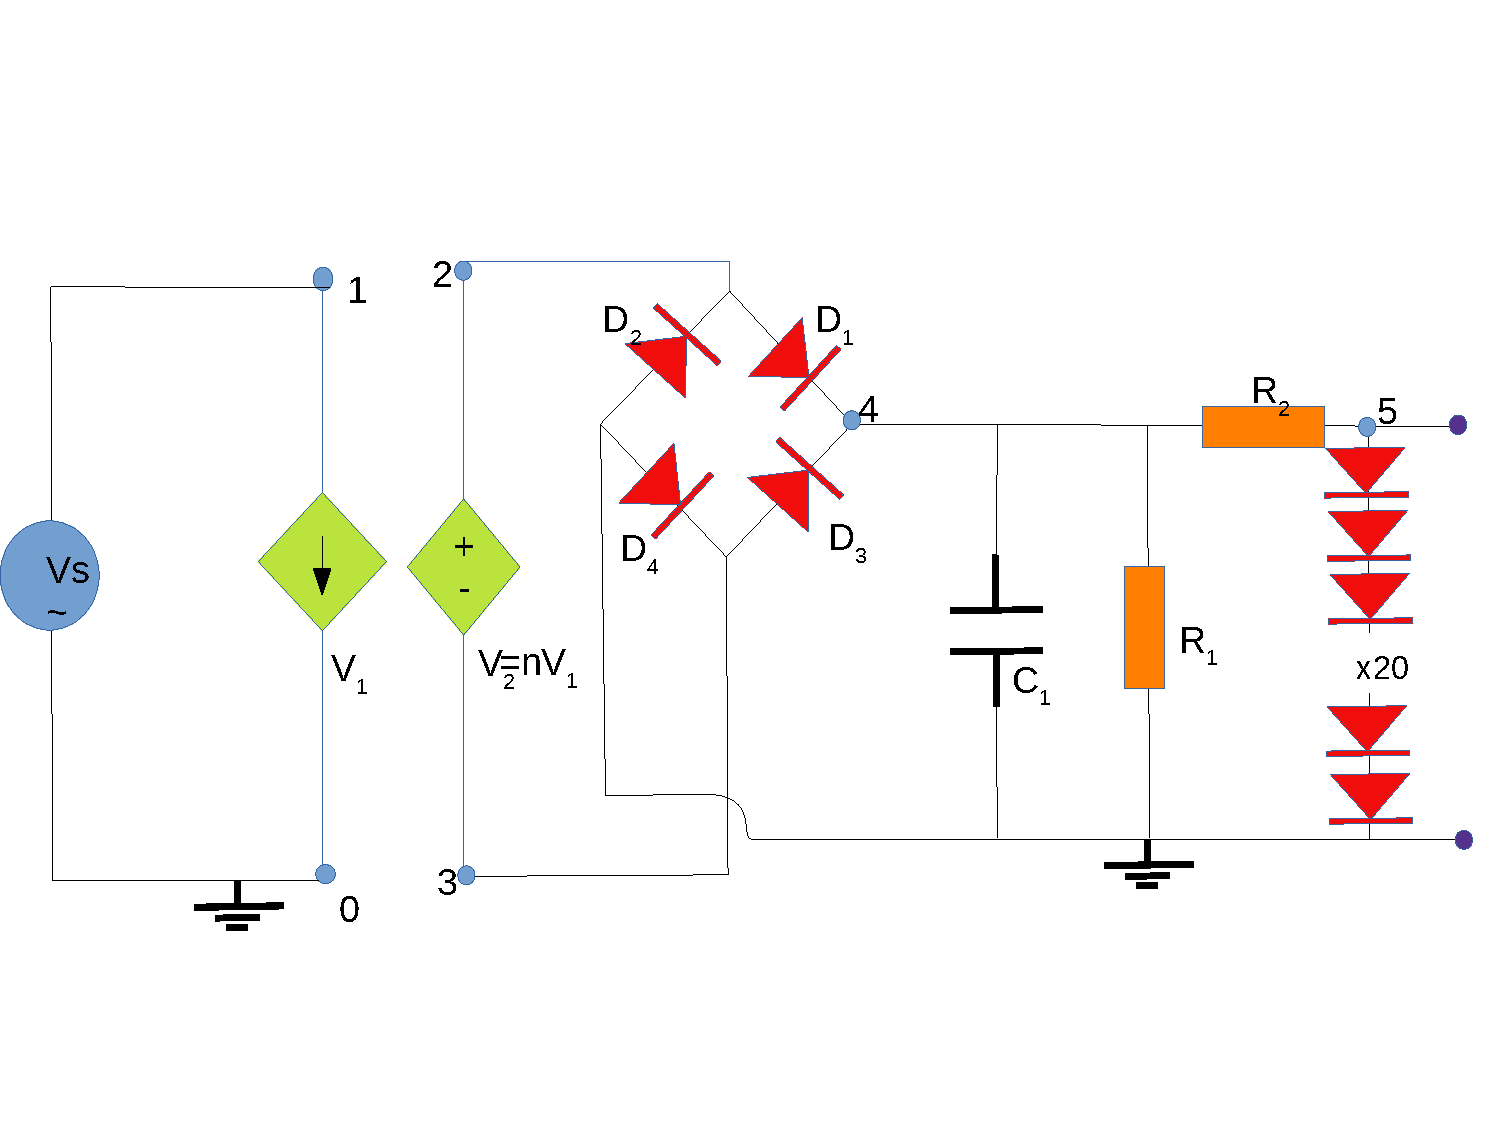
\includegraphics[width=0.8\linewidth]{lab3draw.pdf}
\caption{ AC/DC converter circuit.}
\label{AC/DC circuit.}
\end{figure}
\par 


One method to achieve a steady DC voltage is to use every half-cycle of the input voltage instead of every other half-cycle. The circuit which allows us to do this is called a Full Wave Rectifier. As one may observe, 4 diodes are used, a pair for each half-cycle. Hence, it is completely efficient since it is produced an output for both of them.

In addition, the ripple and voltage variations were reduced by connecting smoothing capacitors. The voltage regulator circuit consists of one resistor and a series of diodes. It keeps the output voltage constant at the desired value (12V) in spite of variations in the supply voltage or in the current load.



\newpage
